% !TEX TS-program = xelatex
% !TEX encoding = UTF-8 Unicode

% Tennessee Technological University
% ME4020 - Fall 2022
% Tristan Hill - November 09, 2022 - October 07, 2024
% Power Screws - This lecture is based on Section 15.2 Power Screws, Machine Design by Norton 6th ed.

\documentclass[fleqn]{beamer} % for presentation (has nav buttons at bottom)

% custom preamble
%\usepackage{/home/tntech.edu/thill/courses/machine_design/machine_design_lecture}
\usepackage{/home/thill/courses/machine_design/machine_design_lecture}


\newcommand{\MNUM}{1\hspace{2mm}} % Module number
\newcommand{\TNUM}{1\hspace{2mm}} % Topic number 
\newcommand{\moduletitle}{Power Screws and Bolted Connections} 
\newcommand{\lecturetitle}{Power Screws} 

\newcommand{\sectiontitleI}{Overview and Applications}
\newcommand{\sectiontitleII}{Threads for Power Transmission}
\newcommand{\sectiontitleIII}{Force and Torque Analysis}
\newcommand{\sectiontitleIV}{Friction and Efficiency}
\newcommand{\sectiontitleV}{ Design Considerations}

\author{ME4020 - Applied Machine Design}
\title{\GD \moduletitle}
\date{Mechanical Engineering\vspc Tennessee Technological University}

\begin{document}

\lstset{language=MATLAB,basicstyle=\ttfamily\small,showstringspaces=false}

\frame{\titlepage \center\begin{framed}\Large \textbf{\lecturetitle}\end{framed} \vspace{5mm}}

% Section 0 - Outline
\frame{
	
	\large \textbf{\lecturetitle} \vspace{3mm}\\
	
	\begin{itemize}
	
		\item \hyperlink{sectionI}{\color{black}\sectiontitleI}	\vspace{3mm} % Section I
		\item \hyperlink{sectionII}{\color{black}\sectiontitleII}	\vspace{3mm} % Section II
		\item \hyperlink{sectionIII}{\color{black}\sectiontitleIII}	\vspace{3mm} %Section III
		\item \hyperlink{sectionIV}{\color{black}\sectiontitleIV}	\vspace{3mm} %Section IV
		\item \hyperlink{sectionV}{\color{black}\sectiontitleV} %Section IV	
	
	\end{itemize}

}

% Section I
\section{\sectiontitleI}

	% Section I - Frame I
	\begin{frame}[label=sectionI] \small
		\frametitle{\sectiontitleI}	

		\begin{multicols}{2}
			A power screw is a machine component that converts rotational motion into linear motion. This is neccesary in variety of applications. 

			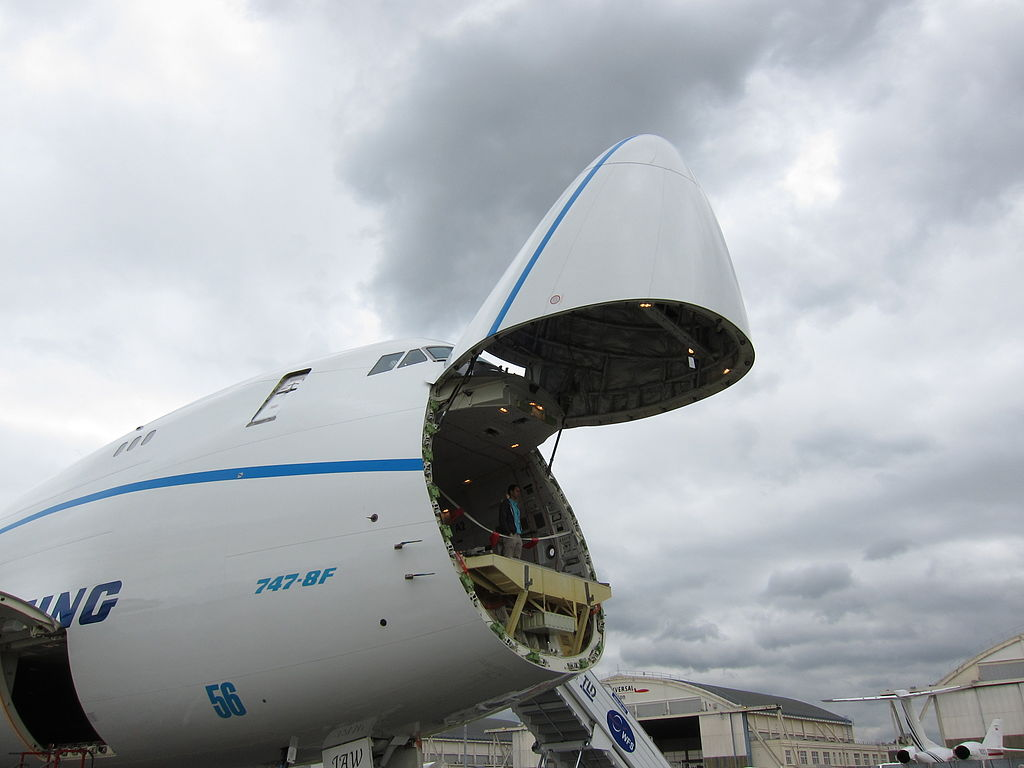
\includegraphics[scale=0.135]{images/1024px-Nose_cargo_door_of_Boeing_747-8F.jpg}

			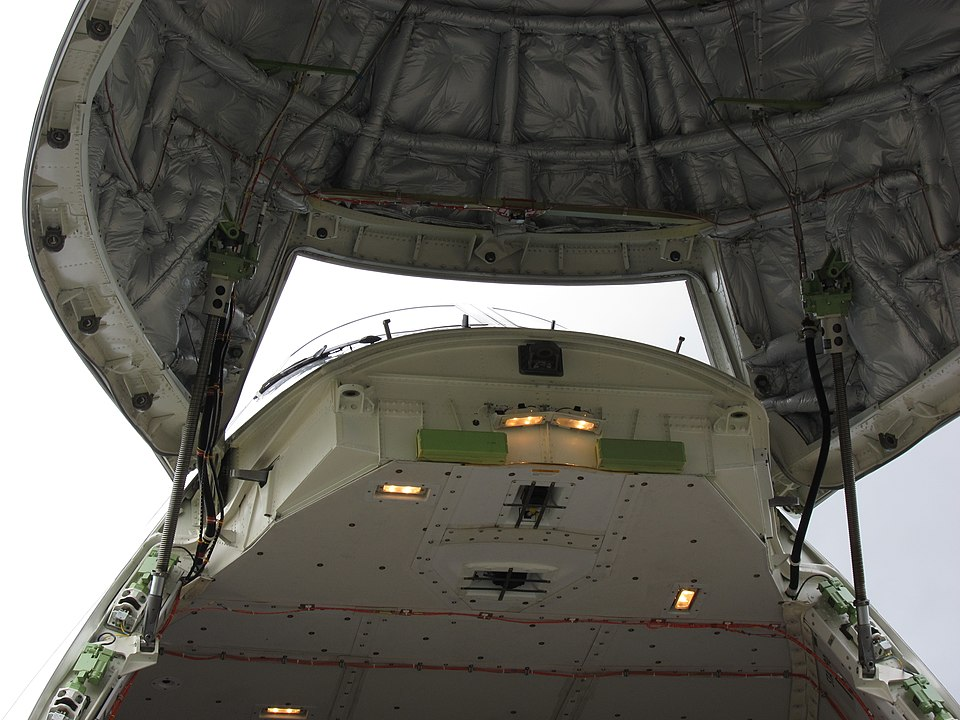
\includegraphics[scale=.175]{images/960px-Detail_of_raised_nose_cargo_door_of_Boeing_747-8F.jpeg}
			\tiny{Leadscrews are used to raise and lower the front door of the Boeing 747-8F Freighter aircraft}
		\end{multicols}

		{\tiny images: \href{https://en.m.wikipedia.org/wiki/File:Nose_cargo_door_of_Boeing_747-8F.jpg}{wikimedia}, \href{https://en.wikipedia.org/wiki/Leadscrew}{wikipedia} }

	\end{frame}


	% Section I - Frame II
	\begin{frame}[label=sectionI] \small
		\frametitle{\sectiontitleI}	
		
		\begin{multicols}{2}
		Common Applications:
		\begin{itemize}
			\item automotive jack and jack post
			\item machining tool positioning
			\item automatic doors and gates 
			\item aircraft control surfaces
			\item automation/production machines	
		\end{itemize}

		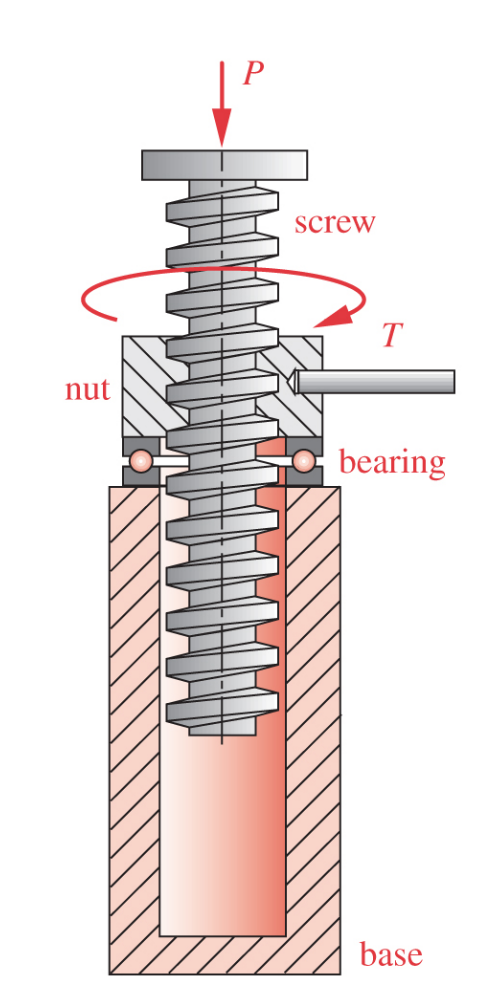
\includegraphics[scale=0.1]{images/figure_15_4.png}
		

		\end{multicols}

	\end{frame}

	% Section I - Frame II
	\begin{frame}[label=sectionI] \small
		\frametitle{\sectiontitleI}	
		Machining Tool Positioning - 3 Axis Mill

		\begin{multicols}{3}
			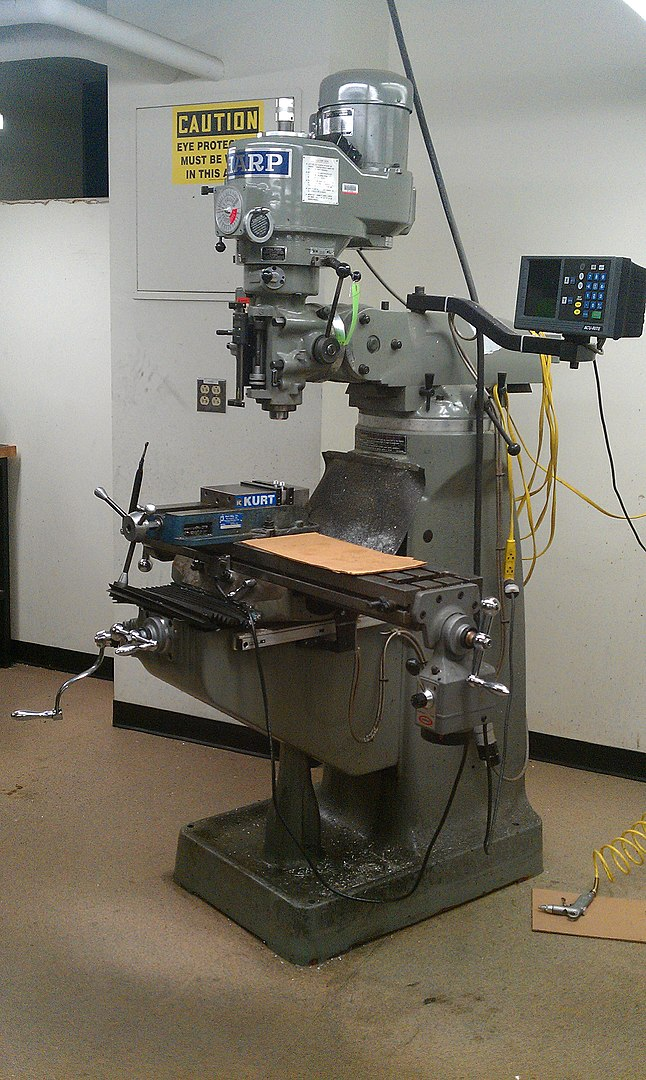
\includegraphics[scale=0.15]{images/Sharp_3_Axis_Vertical_Mill_Full_View.jpeg}

			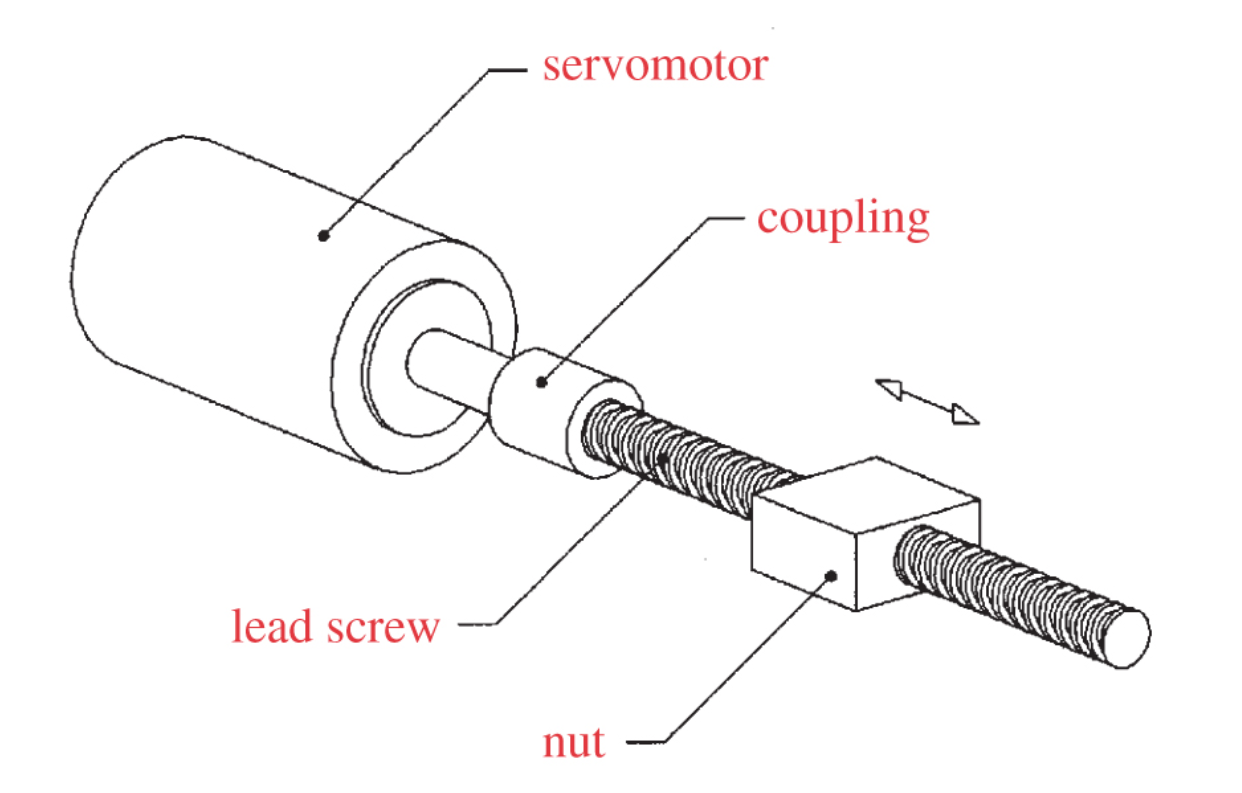
\includegraphics[scale=0.1]{images/figure_15_5.png}

			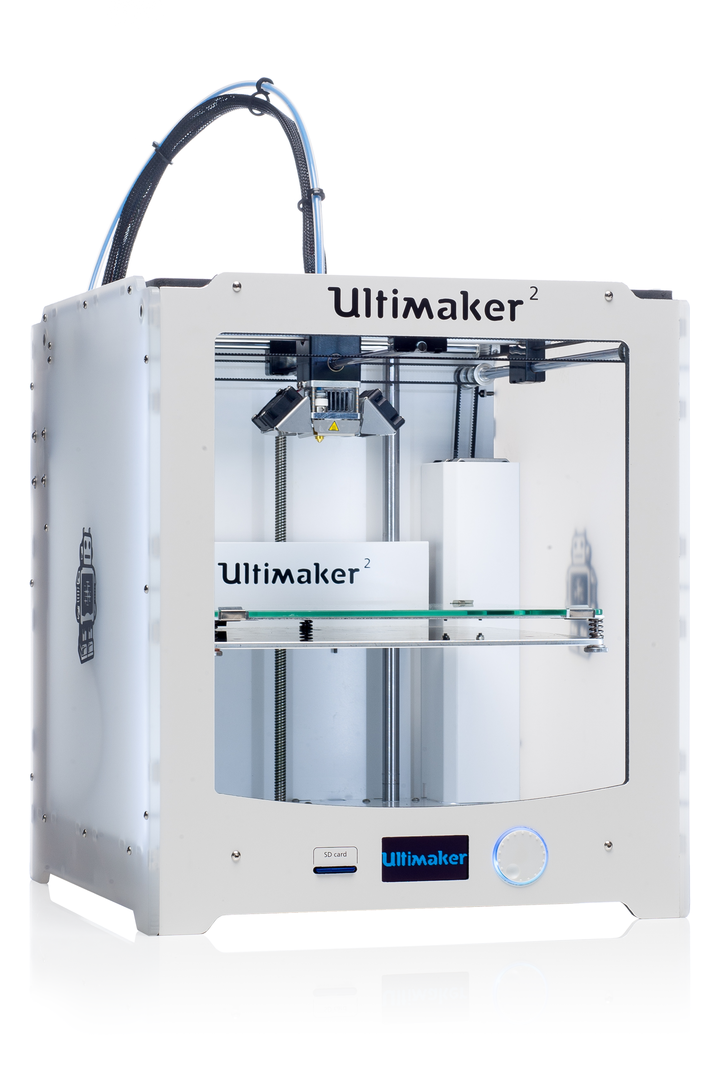
\includegraphics[scale=0.15]{images/Ultimaker_2.png}
		
		\end{multicols}

		\href{https://en.wikipedia.org/wiki/Bridgeport_(machine_tool_brand)\#/media/File:Sharp_3_Axis_Vertical_Mill_Full_View.jpg}{wikipedia: bridgeport}
	
	\end{frame}

	% Section I - Frame III
	\begin{frame}[label=sectionI] \small
		\frametitle{\sectiontitleI}	
		Linear Actuator - General Purpose Machine Component

		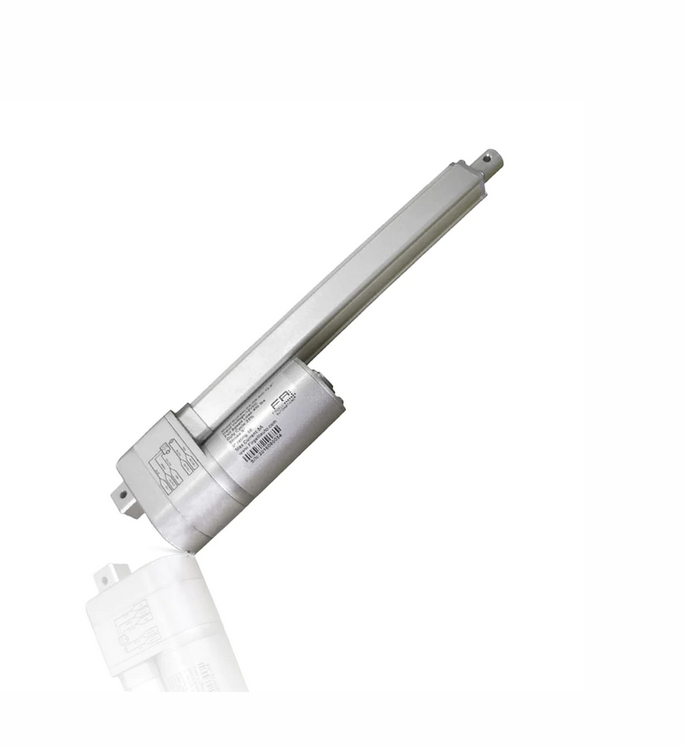
\includegraphics[scale=0.2]{images/fergelli_optical_feedback_actuator.png}

		\href{https://en.wikipedia.org/wiki/Linear_actuator\#/media/File:Linear_actuator_basic.gif}{wikipedia: animation}

	\end{frame}





	% Section I - Frame III
	\begin{frame}[label=sectionI] \small
		\frametitle{\sectiontitleI}	
		
		Advantages:
		\begin{itemize}
			\item large mechanical advantage possible
			\item capable of lifting or moving large loads 
			\item suitable for precision motion control
			\item self locking or back-drivable 
		\end{itemize}

		Disadvantages:
		\begin{itemize}
			\item Low Efficiency due to high friction
			\item High wear possible	
		\end{itemize}

	\end{frame}







% Section II
\section{\sectiontitleII}	

	% Section II - Frame I
	\begin{frame}[label=sectionII] \small
		\frametitle{\sectiontitleII}

		
		\begin{multicols}{2}
		The standard thread form is not strong enough for high load applications. Many power screw applications use a square, acme, or other type of thread for power transmission. \vspace{10mm}

		UN and ISO Standard Thread Form
		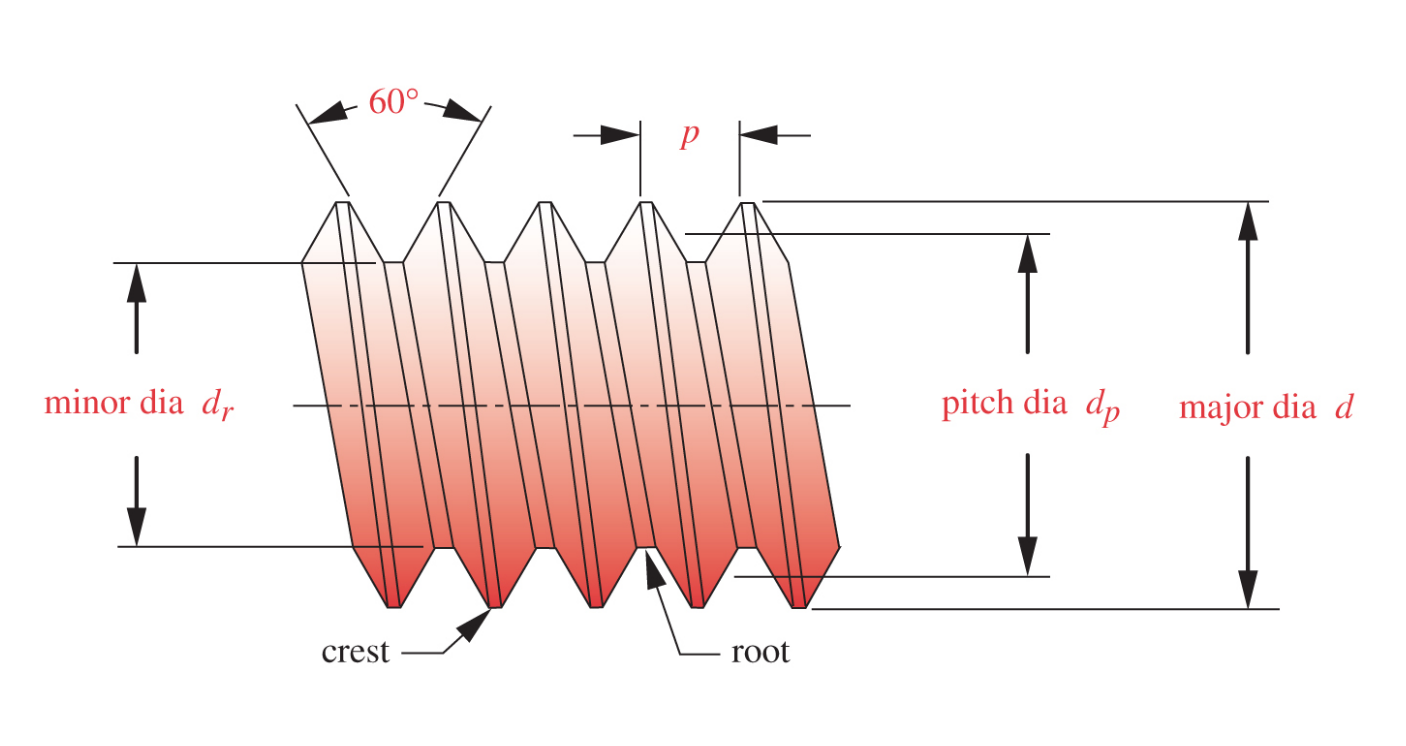
\includegraphics[scale=.1]{images/figure_15_2.png}
		\end{multicols}	

		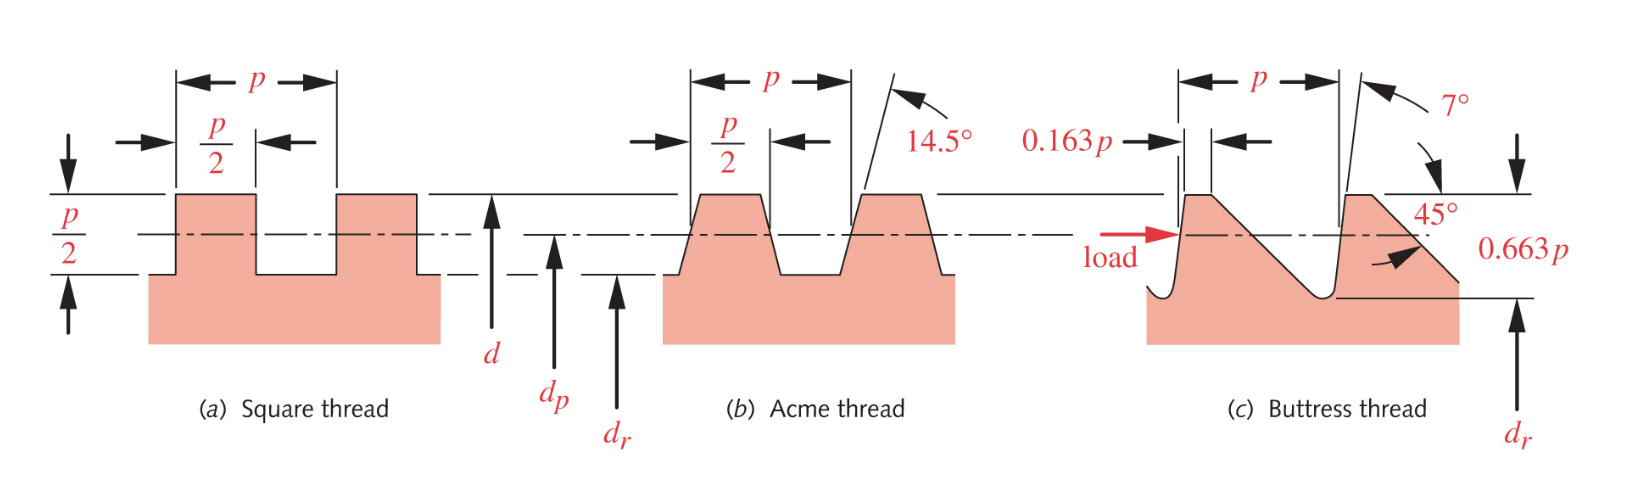
\includegraphics[scale=.15]{images/figure_15_3.png}	

	\end{frame}

	% Section II - Frame II
	\begin{frame}[label=sectionII] \small
		\frametitle{\sectiontitleII}

		Lubrication is required for smooth operation and to avoid excessive wear.

		Ball Screws are used to reduce friction. This adds mechanical complexity, but can increase machine life.

		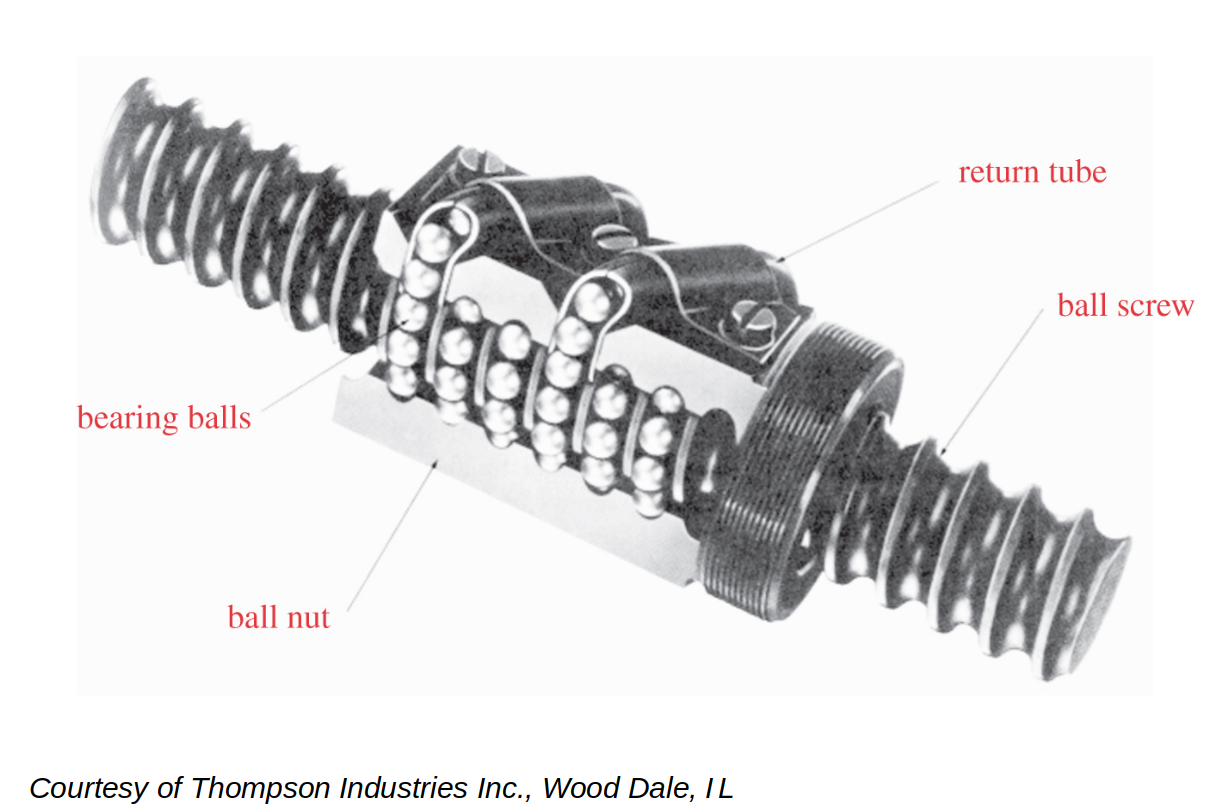
\includegraphics[scale=.15]{images/figure_15_9.png}

	\end{frame}

	% Section II - Frame III
	\begin{frame}[label=sectionII] \small
		\frametitle{\sectiontitleII}
		
	
	\end{frame}

	
% Section III
\section{\sectiontitleIII}	

	% Section III - Frame I
	\begin{frame}[label=sectionIII] \small
		\frametitle{\sectiontitleIII}
	 		
	 	Consider unwinding a single rotation of a square thread. The nut and power screw can be modeled as a block in contact with an inclined plane as shown in the image.	
		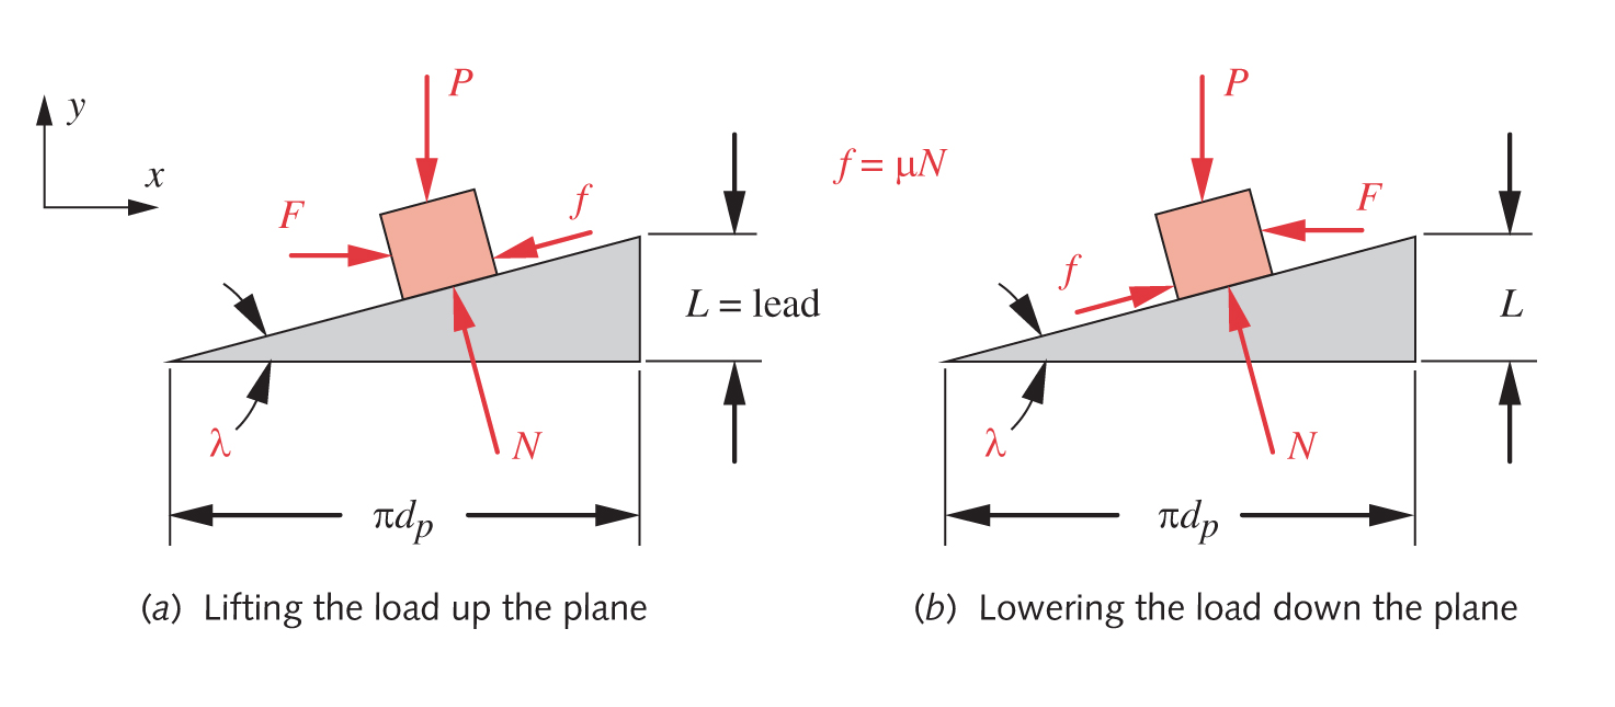
\includegraphics[scale=.15]{images/figure_15_6.png}

		The {\bf lead angle $\lambda$} can be easily found as: 
		\[ tan(\lambda) =\frac{L}{\pi d_p} \implies \lambda = atan(\frac{L}{\pi D_p}) \]
	        
	\end{frame}  

	% Section III - Frame I
	\begin{frame}[label=sectionIII] \footnotesize
		\frametitle{\sectiontitleIII}
		
		\begin{multicols}{2}
			Write the equations of static equillibrium for the lifting case.

			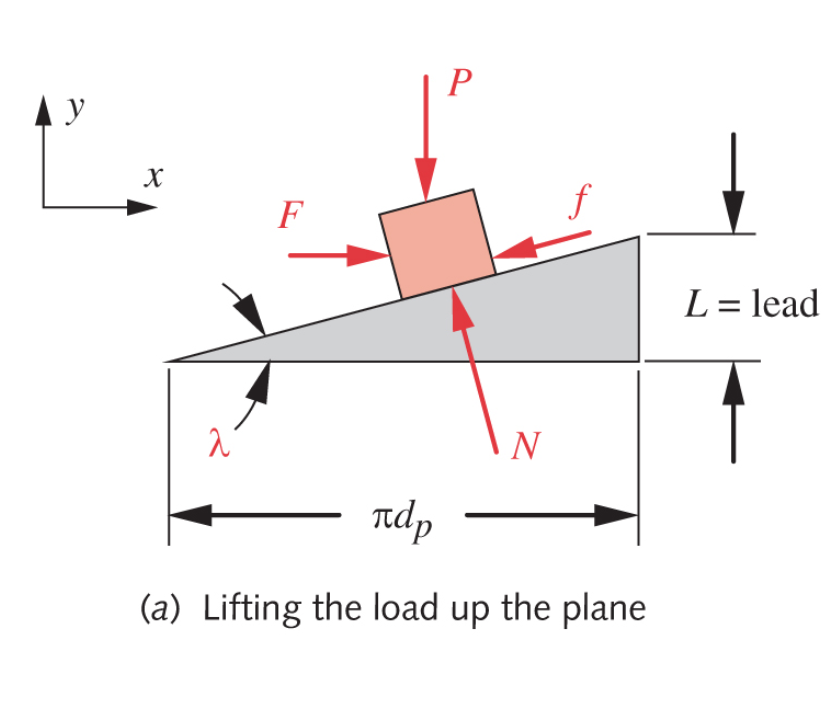
\includegraphics[scale=.12]{images/figure_15_6_a.png}
		\end{multicols}

			\[\Sigma F_x = 0 = F - f cos\lambda -N sin\lambda = F - \mu N cos\lambda - N sin\lambda \]	
			\[F=N(\mu cos\lambda-sin\lambda)\]	

			\[\Sigma F_y = 0 = N cos\lambda - f sin\lambda - P = N cos\lambda -\mu N sin\lambda - P \]
			\[N=\frac{P}{cos\lambda - \mu sin\lambda}\]
	        
	\end{frame}  

	% Section III - Frame I
	\begin{frame}[label=sectionIII] \footnotesize
		\frametitle{\sectiontitleIII}
	 		
		Combine the results of the previous equations to get an expression relating the forces on the nut. The relationship is dependent on the friction coeffient and lead angle of the screw. 

		\[F = P \left( \frac{\mu cos\lambda +sin\lambda}{cos\lambda - \mu sin \lambda} \right)\]
		
		The screw torque required to lift the load can be found as the force in the x direction F times the half pitch diameter.  	

		\[T_{s_u} = F \frac{d_p}{2} = \frac{Pd_p}{2} \left( \frac{\mu cos\lambda +sin\lambda}{cos\lambda - \mu sin \lambda} \right) =  \frac{Pd_p}{2}\left(\frac{\mu \pi d_p +L}{\pi d_p -\mu L} \right) \] 

		The torque required to turn the collar must also be modeled with $d_c$ as the mean diameter and $\mu_c$ as the thrust bearing coefficient

		\[T_c=\mu_cP\frac{d_c}{2}\]

	\end{frame}  

	% Section III - Frame I
	\begin{frame}[label=sectionIII] \footnotesize
		\frametitle{\sectiontitleIII}

		The total torque required to lift the load with a square thread is given as follows:

		\[T_u = T_{s_u}+T_c = \frac{Pd_p}{2}\left(\frac{\mu \pi d_p +L}{\pi d_p -\mu L}\right) + \mu_c P \frac{d_c}{2} \]

		The torque required to lower the load can be found through a similar analysis.

		\[T_d = T_{s_u}+T_c = \frac{Pd_p}{2}\left(\frac{\mu \pi d_p -L}{\pi d_p +\mu L}\right) + \mu_c P \frac{d_c}{2} \]

	\end{frame}


	% Section III - Frame I
	\begin{frame}[label=sectionIII] \footnotesize
		\frametitle{\sectiontitleIII}

		The results for a ACME thread are shown below which include the influence of the angle alpha.

		The total torque required to lift the load with a ACME thread is given as follows:

		\[T_u = T_{s_u}+T_c = \frac{Pd_p}{2}\left(\frac{\mu \pi d_p +L cos \alpha }{\pi d_p cos \alpha-\mu L}\right) + \mu_c P \frac{d_c}{2} \]

		The torque required to lower the load can be found through a similar analysis.

		\[T_d = T_{s_u}+T_c = \frac{Pd_p}{2}\left(\frac{\mu \pi d_p -Lcos \alpha}{\pi d_p cos \alpha +\mu L}\right) + \mu_c P \frac{d_c}{2} \]

		If $\alpha=0$ these will reduce to the equations derived for the square thread.

	\end{frame}


		% Section III - Frame I
	\begin{frame}[label=sectionIII] \footnotesize
		\frametitle{\sectiontitleIII}

		Given the friction coeffients, A force balance can also be used to predict whether the system can be back-driven or not. A power screw which cannot be rotated by any amount of axial load is called {\it self-locking}, which is a useful characteristic in many applications. Power screws that are not self-locking require constant motor input and or a break to hold the system in place. \vspace{5mm}\\

		A screw will {\bf self-lock} if: \[ \mu \geq \frac{L}{\pi d_p}cos\lambda  \hspace{10mm}OR\hspace{10mm}  \mu \geq tan\lambda cos\alpha \]

		for a square thread this becomes: \[\mu \geq \frac{L}{\pi d_p} \hspace{10mm}OR\hspace{10mm} \mu \geq tan\lambda\]


	\end{frame}	
	
	
% Section IV	
\section{\sectiontitleIV}	

	% Section IV - Frame I
    \begin{frame}[label=sectionIV] \small
		\frametitle{\sectiontitleIV}    

		The efficiency of the system is defined as the ratio of {\it work out} to {\it work in}. 

		The work done on the power screw is the torque times the angular displacement in radians. For a single rotation this is given as: 

		\[W_{in}=2\pi T\]

		The work delivered through one revolution is the load force times the lead.

		\[W_{out}=PL\]

		The efficiency of the system is:

		\[e=\frac{w_{out}}{W_{in}}=\frac{PL}{2\pi T} = \frac{1-\mu tan\lambda}{1+\mu cot\lambda}\]

	\end{frame}


	% Section IV - Frame I
    \begin{frame}[label=sectionIV] \small
		\frametitle{\sectiontitleIV}  	

		Efficiency of an ACME-Thread at different lead angles and coefficients of friction.

		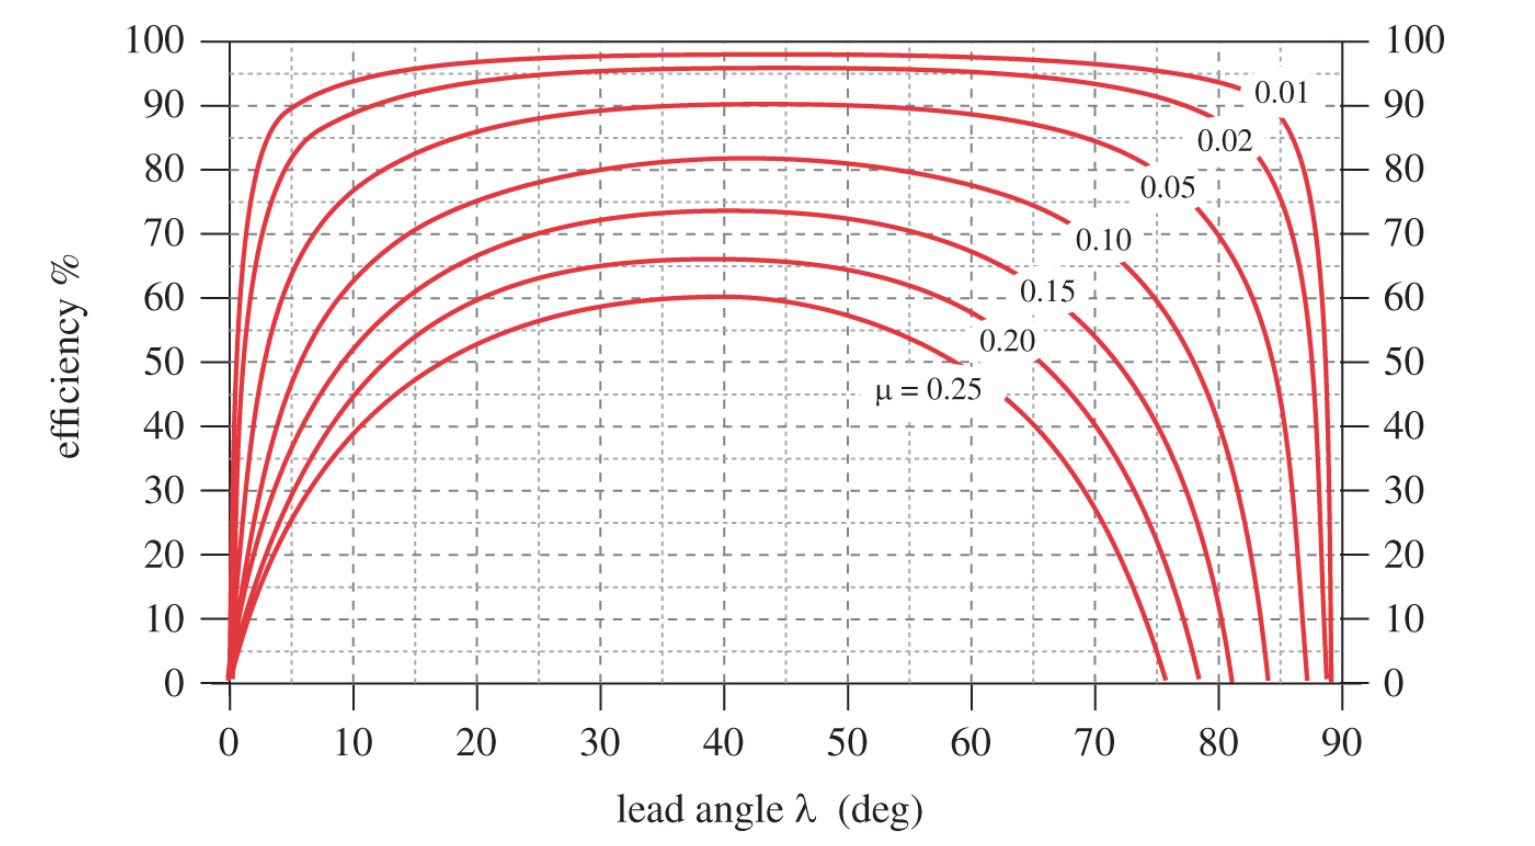
\includegraphics[scale=.2]{images/figure_15_8.png}



	\end{frame}



		

% Section V	
\section{\sectiontitleV}	

	% Section V - Frame I
    \begin{frame}[label=sectionV] \small
	\frametitle{\sectiontitleV}    

  	

	\end{frame}

	% Section V - Frame II
    \begin{frame}[label=sectionV] \small
  

	References: \vspace{10mm} \\

	This lecture was adapted from \underline{Machine Design} by Norton, 6th ed. Section 15.3 \vspace{10mm} \\
	
	Images are from the above textbook and wikipedia/wikimedia.

	\end{frame}
		
\end{document}